% Much of these are still open because I haven't leveraged more recent (i.e. better) data.  So worth re-doing the analysis with it (I have better data & I'm better at coding & after writing this I see how it all fits together).

% Does it make sense to introduce methods (plus investigations, specifically for ACF/XCF) BEFORE describing the whole 'pipeline'?  This chapter is getting unwieldy, especially when I go back and forth between the mathematical methods.
\chapter{Analysis of oscillatory time series in the yeast metabolic cycle}
\label{ch:analysis}

To characterise the properties of large sets of time series generated by microfluidics experiments, I sought to develop a pipeline of time series analysis methods.

Short and noisy oscillatory time series are challenging to analyse to give usable characteristics such as period and phase, especially because of the limited information they encode.
To illustrate the challenge, microfluidics experiments capture up to 5--10 periods metabolic cycles, so Fourier analysis gives period estimates at low resolution.
In addition, there is no standard method of analysing oscillatory time series such as those that arise from the yeast metabolic cycle.

Here, I propose steps for the analysis of datasets of 100--1000 time series related to the yeast metabolic cycle from single cells, using my experimental data as an example case.

Specifically, I address:
\begin{enumerate}
  \item Cleaning: choosing data and filtering out long-term trends that may confound further analysis.
  \item Classification: determining whether a time series exhibits oscillations.
  \item Characterisation: identifying the properties of a single time series, with an emphasis on the period and noise quality.
  \item Correlation: identifying the relationship between two types of signal from the same cell.
  \item Clustering: identifying the relationship between multiple time series of the same type of signal from a population of cells.
        Such a relationship may include groupings or structures within the population of time series.
\end{enumerate}

In this chapter, I will ... (REVISIT THIS AFTER I GO THROUGH EVERYTHING)


\section{Analysing time series in a biological context}
\label{sec:analysis-literature}

Previous studies have described mathematical and computational methods to analyse biological time series.

\textcite{zielinskiPeriodEstimationRhythm2022} described a software pipeline (BioDare/BioDare2) to estimate the period and detect rhythms in time series catered to circadian rhythm studies.
This pipeline includes choices of detrending and normalising data, followed by a choice of methods to estimate the period, phase, and amplitude of the time series.
Furthermore, the pipeline also includes an implementation of the JTK\_CYCLE test \parencite{hughesJTK_CYCLEEfficientNonparametric2010} along with an empirical derivative \parencite{hutchisonImprovedStatisticalMethods2015a} as statistical tests for the presence of an oscillation in a time series.

BioDare2 builds upon \textcite{zielinskiStrengthsLimitationsPeriod2014}, which compared and contrasted a set of period-estimation methods ---
% shopping-list?
% Also: define these/add citations
FFT-NLLS, mFourFit, MESA, the Enright periodogram, the Lomb-Scargle periodogram, and spectrum resampling --- to conclude with recommendations on time series analysis.
These recommendations include:
\begin{enumerate}
  \item \emph{Amount of data:} To determine whether a time series is oscillatory, at least 2.5 cycles are needed.
        To estimate the period to within \SI{0.5}{\hour} for a \SI{24}{\hour} period, at least 5 cycles are needed.
  \item \emph{Data pre-processing:} Baseline trends must be removed.
  \item \emph{Detecting rhythmicity:} The Enright periodogram can be used.
  \item \emph{Estimating period:} mFourFit and MESA should be used as a minimum and agreement between the two methods is a good indicator of accuracy because the methods are based on different principles.
        Additionally, FFT-NLLS can be used to provide error measures for the period, phase, and amplitude.
\end{enumerate}

Studies of biological rhythms have used the BioDare pipeline to quantify features of oscillations of fluorescence.
These include using FFT-NLLS to calculate the period and amplitude error of fluorescence in mouse brain sections to determine the mechanistic basis of the synchronisation of the suprachiasmatic nucleus \parencite{hamnettVasoactiveIntestinalPeptide2019}, and using linear detrending of data followed by FFT-NLLS and spectral resampling to estimate the period and amplitude error of delayed fluorescence of chloroplasts in \textit{Kalancho\"{e} fedtschenkoi} leaves to determine whether phosphorylation of phosphoenolpyruvate affects robustness of circadian rhythms.

As another example, \textcite{fulcherHctsaComputationalFramework2017} described a software pipeline, termed \textit{hctsa}, that computes over 7700 time series features for input time series.
The resulting feature matrix --- a row for each time series and a column for each feature --- could then be used to identify sets of features that are useful to discriminate between sets of time series that corresponding to biological groups, or to identify clusters of time series based on their properties.
The publication then showed that \textit{hctsa} could be used to distinguish five \textit{Caenorhabditis elegans} strains based on their movement patterns, and to identify clusters in the feature space of time series of \textit{Drosophila melanogaster} movement patterns which correspond well to experimental groups.
To reduce computation time, \textcite{lubbaCatch22CAnonicalTimeseries2019} identified 22 features, termed \textit{catch22}, of \textit{hctsa} that performed well in time series classification tasks based on 93 datasets.

Taken together, the two examples of BioDare and \textit{hctsa} demonstrate two approaches to analysis of time series: on one end, relying on mathematical methods, and on the other end, a data science approach to time series classification tasks.


\section[Cleaning]{Cleaning: choosing data, filtering out long-term trends}
\label{sec:analysis-cleaning}

Biological time series often have long-term trends that are not useful and may confound analysis.
In my study of the yeast metabolic cycle, such trends include slow, global changes in flavin autofluorescence, which must be removed to uncover the periodic behaviour of flavin autofluorescence that is a component of the metabolic cycle.
To determine the detrending method that is most appropriate for my data, I compared a frequency filtering method, a sliding-window detrending method, and a polynomial detrending method.

\textcite{zielinskiPeriodEstimationRhythm2022} describes several methods of detrending time series:
% Clarify definitions -- this is currently like a shopping list.
\begin{enumerate}
  \item Polynomial detrending (including cubic linear detrending)
  \item Sliding-window detrending (termed as baseline detrending)
  \item Amplitude-and-baseline detrending (modifies sliding-window detrending by remove amplitude dampening)
\end{enumerate}

However, each method has its own caveats.
Polynomial detrending assumes a polynomial-shaped underlying signal, while methods based an sliding-window detrending necessitates discarding time points at the beginning and end of the time series and may introduce strong artefacts.

\begin{figure}
  \centering
  \begin{subfigure}[htpb]{0.8\textwidth}
   \centering
   \includegraphics[width=\textwidth]{fft_raw}
   \caption{
   }
   \label{fig:analysis-filter-raw}
  \end{subfigure}

  \begin{subfigure}[htpb]{0.8\textwidth}
   \centering
   \includegraphics[width=\textwidth]{fft_butterworth}
   \caption{
   }
   \label{fig:analysis-filter-butterworth}
  \end{subfigure}

  \caption{
    (Left panels) Time series and (right panels) Fourier spectra corresponding to
    \textbf{(\ref{fig:analysis-filter-raw})}
    a sample raw time series of flavin autofluorescence, and
    \textbf{(\ref{fig:analysis-filter-butterworth})}
    the time series processed by a high-pass Butterworth filter with a critical frequency \SI[parse-numbers=false]{1/350}{\minute^{-1}}.
  }
  \label{fig:analysis-filter}
\end{figure}

To demonstrate the use of a method that modifies the frequency profile of time series to remove trends, Fig.\ \ref{fig:analysis-filter} shows how a time series and its Fourier spectrum changes after the application of a high-pass Butterworth filter with a critical frequency of \SI[parse-numbers=false]{1/350}{\minute^{-1}}.
Unlike sliding-window methods, defining a signal filter offers direct control over frequencies.
The critical frequency in this case was defined to create a reasonable upper limit of periods of the yeast metabolic cycle, based on my observations in single-cell microfluidics experiments.
Defining this critical frequency is a trade-off between emphasising metabolic oscillations in expected frequency windows and excluding the possibility of long-period metabolic cycles.


\begin{figure}
  \centering
  \begin{subfigure}[htpb]{0.8\textwidth}
   \centering
   \includegraphics[width=\textwidth]{fft_slidingwindow}
   \caption{
   }
   \label{fig:analysis-slidingwindow-movavg}
  \end{subfigure}

  \begin{subfigure}[htpb]{0.8\textwidth}
   \centering
   \includegraphics[width=\textwidth]{fft_savgol}
   \caption{
   }
   \label{fig:analysis-slidingwindow-savgol}
  \end{subfigure}

  \caption{
    (Left panels) Raw time series with trends, (middle panels) processed time series, and (right panels) Fourier spectra to demonstrate
    \textbf{(\ref{fig:analysis-slidingwindow-movavg})}
    using a moving average (window size 30), and
    \textbf{(\ref{fig:analysis-slidingwindow-savgol})}
    using a Savitzky-Golay filter (window size 7, polynomial order 3)
    to remove trends.
  }
  \label{fig:analysis-slidingwindow}
\end{figure}

To show how sliding-window methods adversely affect the frequency profile of time series when used for detrending, I computed the Fourier spectrum of time series detrended using the moving average method and the Savitzky-Golay filter.
Sliding-window methods are common in detrending biological time series.
For example, \textcite{cunyHighresolutionMassMeasurements2022} used a moving average: a constant, defined sliding window to smooth time series of yeast cell mass during growth.
\textcite{papagiannakisAutonomousMetabolicOscillations2017} fitted a smoothing spline to their single-cell fluorescence data of the yeast metabolic cycle, then divided the data points by the smoothing spline to detrend their data; the specific mathematical method used to define the smoothing spline was unclear in their study.
% Equations?
The Savitzky-Golay filter is also common --- this method is based on fitting a sliding window of a defined number of time points with a polynomial of a defined order using least squares fitting.

Fig.\ \ref{fig:analysis-slidingwindow-movavg} shows that the moving average method introduced an artefact in the frequency spectrum near the reciprocal of the window size and decreases the number of time points.
In contrast, Fig.\ \ref{fig:analysis-slidingwindow-savgol} shows that the Savitzky-Golay filter ...(INSERT DISCUSSION HERE)...
In sum, sliding-window methods were not ideal because they distorted the data in a way that affects conclusions, or removed noise information that may be useful.
% Really?
Importantly, it is not possible to restore the raw data when it is processed using such methods.

Therefore, for subsequent analyses, I used the high-pass Butterworth filter defined above to process raw fluorescence time series.
This is because using this method, I obtain more control over the frequency components, and the methods preserves noise frequencies that are useful for assessing the quality of the data set and estimating the noise properties.


\section[Classification]{Classification: is my time series oscillatory?}
\label{sec:analysis-classification}

To assess how a perturbation affects the YMC, it is important to have a systematic method to determine whether a time series is oscillatory.
Determining whether a time series is oscillatory, or rhythmicity detection, is challenging because the task of defining the presence of an oscillation breaks down when the frequency domain is considered.
Rhythmicity detection is best re-defined as identifying the presence of a frequency in a range of interest, excluding lower frequencies that contribute to trends, and higher frequencies that contribute to noise \parencite{zielinskiStrengthsLimitationsPeriod2014}.
However, there is no way to objectively specify a failure rate for a rhythmicity detection method as there is no independent method to estimate rhythmicity; therefore, evaluating such a classification method requires a subjective definition of whether each time series is oscillatory.

To determine the time series classification method that is most appropriate for my data, I compared a  spectral methods, a model-fitting method, and a machine learning method.


\subsection{Rhythmicity detection using spectral methods}
\label{subsec:analysis-classification-spectral}

In order to classify oscillatory and non-oscillatory time series, I modified a classifier based on a spectral method that included a statistical test.
This classifier was based on \textcite{glynnDetectingPeriodicPatterns2006a}, which described a method to classify gene expression profiles as oscillating or non-oscillating based on the Lomb-Scargle periodogram \parencite{lombLeastsquaresFrequencyAnalysis1976}.
This periodogram was developed for time series with missing time points, and has a chi-square distribution that aids a statistical test for periodicity \parencite{scargleStudiesAstronomicalTime1982}.
The classification was based on controlling the false discovery rate for identification of oscillations.
In testing multiple hypotheses, the false discovery rate is defined as the proportion of cases in which the null hypothesis is true among all hypotheses in which the test is declared significant.
Increasing the false discovery rate thus increases the proportion of time series classed as oscillating.

The classifier can be described mathematically as follows:

\begin{enumerate}
\item Let the data have $\mathcal{G}$ cells.
Let cell $g = 1, \dots{}, \mathcal{G}$ have a time series with $N_{g}$ time points.
The time series is thus denoted $Y_{g}(t) = y_{g}(t_{1}), \dots{}, y_{g}(t_{N_{g}})$.
\item For each time series, I define a range of test frequencies linearly from $\frac{1}{N_{g}}$ to the Nyquist limit (i.e. half the rate of image acquisition, \SI{0.2}{\minute^{-1}}, in this case).

With this definition, I compute the classical periodogram for each time series:
  \begin{equation}
    P_{g}(\omega) = \frac{N_{g}}{2\sigma^{2}} \left|\int_{-\infty}^{\infty} Y_{g} e^{-2\pi it}dt \right|, % check constants, etc
    \label{eq:normalised-periodogram-ar}
  \end{equation}
        where $\sigma^{2}$ is the sample variance of $Y_{g}$.
        In this equation, the periodogram is normalised by the coefficient $N_{g}/2\sigma^{2}$ so that the area under the periodogram is constant across all time series.
        The Lomb-Scargle periodogram is equivalent to the classical periodogram if the time points are equally spaced \parencite{lombLeastsquaresFrequencyAnalysis1976}, as is the case for the vast majority of my data.
\item For each cell $g$, I denote the peak $h_{g} = \max_{j}P_{g}(\omega)$.
I define an effective number of independent frequencies $M = f_{max}N_{g}$ for each time series, where $f_{max}$ is the Nyquist limit \parencite{vanderplasUnderstandingLombScarglePeriodogram2018}.
  I then calculate the $p$-value of testing the null hypothesis that such a peak is due to chance:
  \begin{equation}
    p_{g} = 1 - (1 - e^{-h_{g}})^M
    \label{eq:lsp-pval}
  \end{equation}
  This formula is based on the exponential distribution of the power at a given frequency in the periodogram \parencite{scargleStudiesAstronomicalTime1982}.
\item I order the cells by $p$-values: $p_{(1)} \leq p_{(2)} \leq \dots \leq p_{(\mathcal{G})}$.
  To control the false discovery rate \parencite{benjaminiControllingFalseDiscovery1995}, I find $\hat{k}$ according to:
  \begin{equation}
    \hat{k} = \arg\max_{1 \leq k \leq \mathcal{G}}\{k : p_{(k)} \leq qk/\mathcal{G}\}
    \label{eq:lsp-khat}
  \end{equation}
  where $q$ is a defined false discovery rate.
\item Cells whose $p$-values correspond to $p_{(1)}, p_{(2)}, \dots, p_{(\hat{k})}$ are thus denoted to have statistically significant oscillatory behaviour for the false discovery rate $q$.
\end{enumerate}

Subsequently, the peak of the normalised classical periodogram of each time series was used as a proxy for the quality of oscillation, and therefore, the time series can be rank according to the height of this peak.


\begin{figure}[htbp]
  \centering
  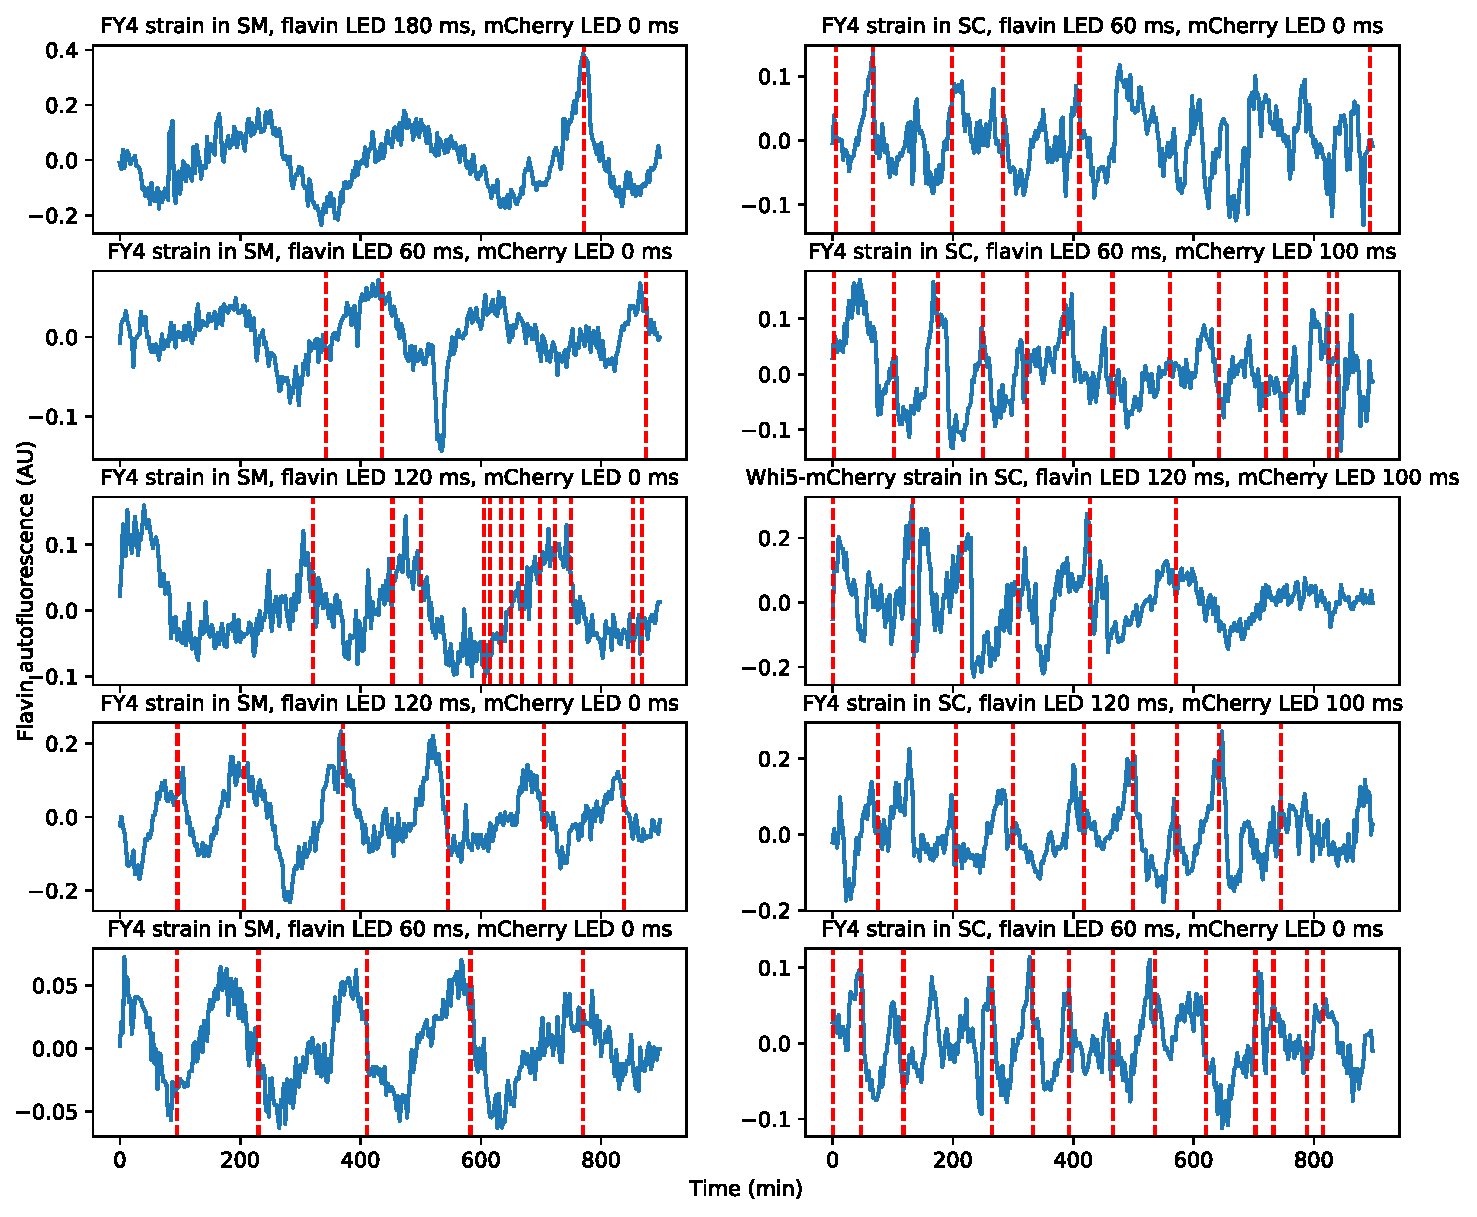
\includegraphics[width=\textwidth]{10m_ClassifierBestWorstTS}
  \caption[
    Classifier based on Lomb-Scargle periodogram ranks time series by quality of oscillation
  ]{
    Classifier based on Lomb-Scargle periodogram ranks time series by quality of oscillation.
    Left column shows `best' five and right column shows `worst' five.
    Blue solid lines: flavin autofluorescence, red dashes: birth event automatically identified by \textit{BABY}.
  }
  \label{fig:ClassifierBestWorstTS}
\end{figure}

\begin{figure}[htbp]
  \centering
  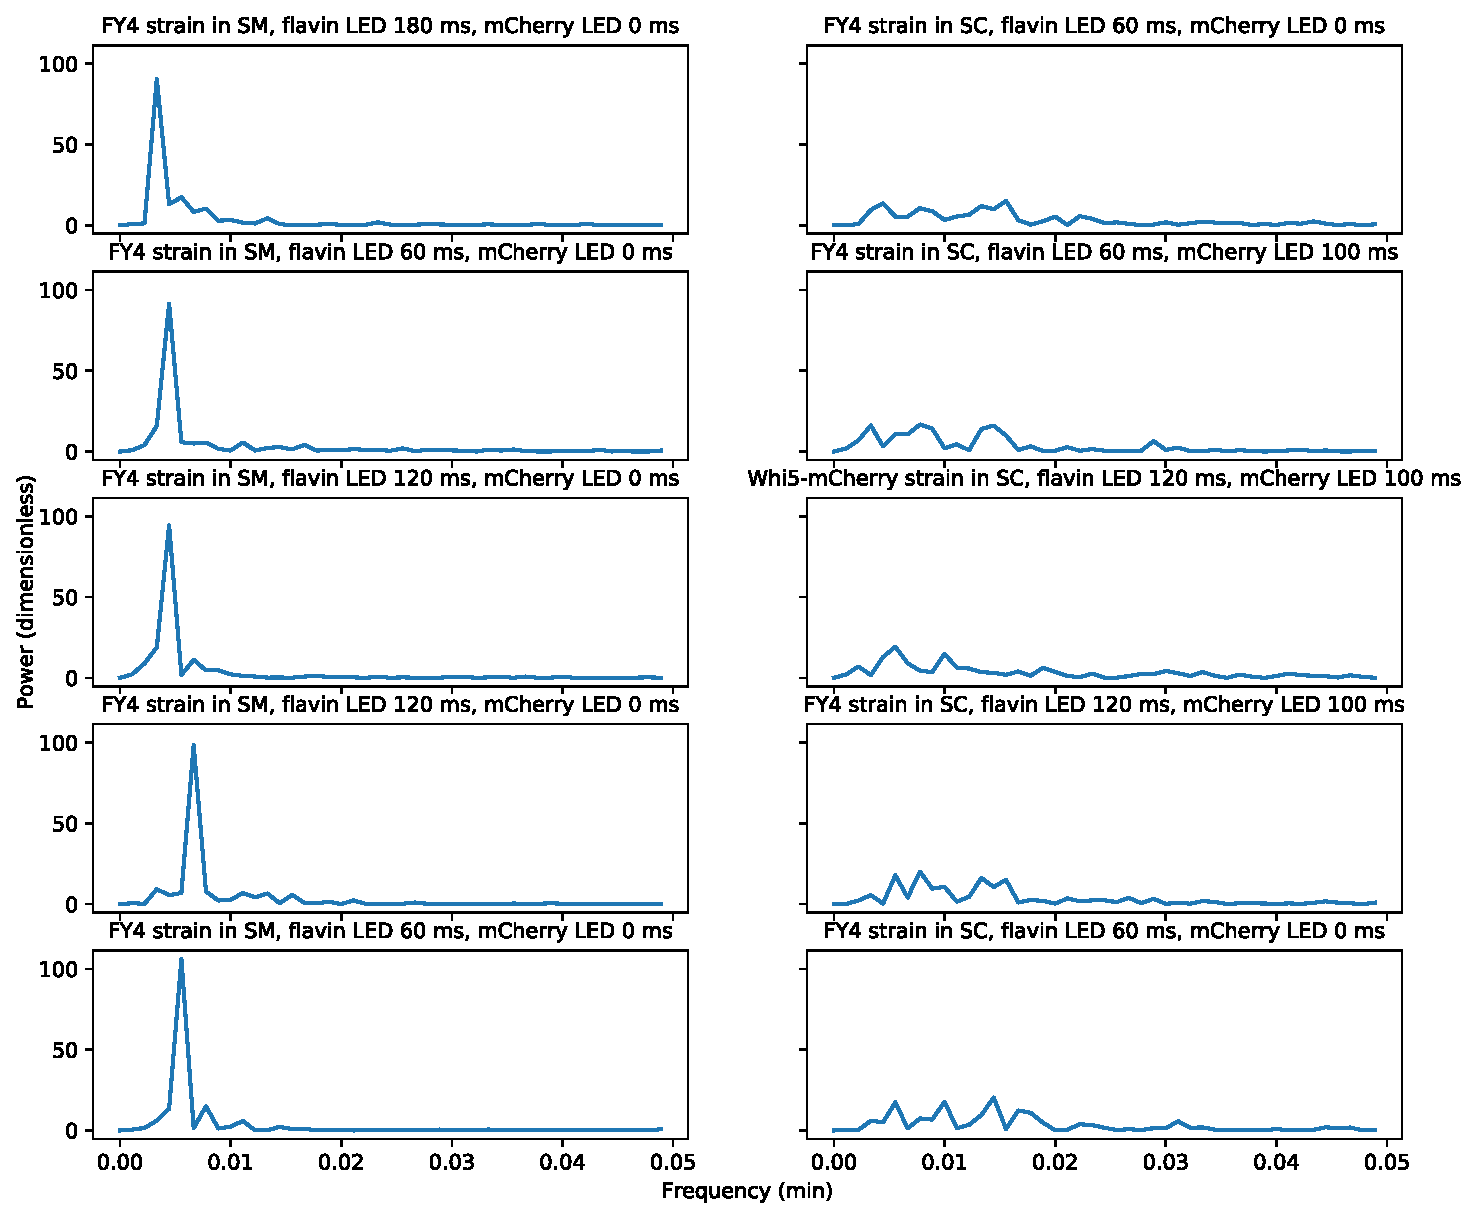
\includegraphics[width=\textwidth]{10m_ClassifierBestWorstPS}
  \caption[
    Highest peak of normalised classical periodograms is an inadequate proxy for quality of oscillations
  ]{
    Highest peak of normalised classical periodograms is an inadequate proxy for quality of oscillations.
    Blue solid lines: normalised classical periodograms of time series in figure \ref{fig:ClassifierBestWorstTS}.
  }
  \label{fig:ClassifierBestWorstPS}
\end{figure}

Fig.\ \ref{fig:ClassifierBestWorstTS} shows that the classifier correctly ranked high-quality oscillations, determined subjectively, as the highest-quality oscillations.
However, the time series that it ranked as lowest-quality exhibited oscillations, albeit at a higher frequency, as informed, subjectively, by the coincidence of regular budding events with peaks in the oscillations.
These oscillations were ranked as low-quality because the Fourier spectrum (Fig.\ \ref{fig:ClassifierBestWorstPS}) identified multiple main frequencies, and thus lowered the peak of the normalised periodogram.
Thus, a Fourier-based method may not adequately provide the information for a reliable ranking of oscillation quality.

Another caveat of this classifier lies in its sole tuning parameter, the false discovery rate, which affects the proportion of time series classed as oscillating.
To optimise the false discovery rate, labels of whether a time series is oscillatory were needed; if the labels are human-defined, as was the case in this section, any optimised false discovery rate would have low reliability.
Alternatively, a more reliable ground truth could be provided by an experiment expected to result in time series that are not oscillatory.


\subsection{Rhythmicity detection using model fitting}
\label{subsec:analysis-classification-ar}

To identify an alternative method to classify oscillatory and non-oscillatory time series, I assessed the performance of a time series classification method based on the autoregressive model.
%The autoregressive model has been used before to characterise biological time series \parencite{zielinskiStrengthsLimitationsPeriod2014}.
This type of model is based on the assumption that each data point in the time series can be expressed as a linear combination of $P$ data points that precede it, thus smoothing the time series.
The advantage of the autoregressive model is that it leads to an analytical solution for the periodogram, thus potentially resolving the problem of a low-resolution periodogram based on the Fourier spectrum.

In particular, \textcite{jiaFrequencyDomainAnalysis2021} describes a model of stochastic gene expression in a dividing cell, which predicts oscillatory gene expression.
Autoregressive models were fitted to simulated time series of oscillatory gene expression, and its parameters used to define a power spectrum for the time series.
This model-fitting can be described mathematically as follows:

\begin{enumerate}
  \item The algorithm relies on fitting a single time series $n(0), n(1), \ldots , n(M-1)$ with an autoregressive model $\mathrm{AR}(P)$ with order $P$:
        \begin{equation}
          \label{eq:ar-model}
          \phi_{0}n_{t} + \phi_{1}n_{t-1} + \phi_{2}n_{t-2} + \ldots + \phi_{P}n_{t-P} = \theta_{0}\epsilon_{t}
        \end{equation}
        where $\epsilon_{t}$ is a white noise satisfying $\langle \epsilon_{t} \rangle = 0$,
        $\phi_{0} = 1$, and
        $\phi_{1}, \ldots , \phi_{P}$ are real numbers such that the complex zeros of the polynomial $\Phi (z) = \sum_{k=0}^{P} \phi_{k}z^{k}$ lie outside the unit circle.
  \item The sample mean of the time series is estimated by:
        \begin{equation}
          \label{eq:ar-mean}
          \langle n \rangle = \frac{1}{M} \sum_{k=0}^{M-1}n(k)
        \end{equation}
  \item The sample autocorrelation function is estimated as:
        \begin{equation}
          \label{eq:ar-acf}
          R_{i} = \frac{1}{M} \sum_{k=0}^{M-1-i}(n(k) - \langle n \rangle)(n(k+i) - \langle n \rangle)
        \end{equation}
  \item The coefficients $\phi_{1}, \ldots , \phi_{P}$ are estimated by solving the Yule-Walker equation:
        \begin{equation}
          \label{eq:ar-yule-walker}
          \begin{bmatrix}
            R_{0} & R_{1} & \dots & R_{P-1} \\
            R_{1} & R_{0} & \dots & R_{P-2} \\
            \vdots & \vdots & \ddots & \vdots \\
            R_{P-1} & R_{P-2} & \dots & R_{0}
          \end{bmatrix}
          \begin{bmatrix}
            \phi_{1} \\
            \phi_{2} \\
            \vdots \\
            \phi_{P}
          \end{bmatrix}
          =
          \begin{bmatrix}
            R_{1} \\
            R_{2} \\
            \vdots \\
            R_{P}
          \end{bmatrix}
        \end{equation}
  \item The parameter $\theta_{0}$ is estimated as:
        \begin{equation}
          \label{eq:ar-noise-param}
          \theta_{0}^{2} = R_{0} - \sum_{k=1}^{P}\theta_{k}R_{k}
        \end{equation}
  \item The order $P$ is determined by minimising the Akaike information criterion:
        \begin{equation}
          \label{eq:ar-aic}
          \mathrm{AIC}(P) = \log \theta_{0}^{2}(P) + 2 \frac{P}{M}
        \end{equation}
        where $\theta_{0}(P)$ is the estimated $\theta_{0}$ (equation~\ref{eq:ar-noise-param}) for a specific $P$.
        In this step, $P$ is varied with $1 \leq P \leq 3 \sqrt{M}$, and the optimum order ($P$) is the one that gives the smallest value of $\mathrm{AIC}(P)$
   \item The power spectrum is thus estimated analytically using the parameters found in earlier steps by:
        \begin{equation}
          \label{eq:ar-power-spectrum}
          G(\xi) = \frac{1}{2 \pi} \cdot \frac{\theta_{0}^{2}}{|\sum_{k=0}^{P}\phi_{k}\me^{-ik\xi}|^{2}}, -\pi \leq \xi \leq \pi
        \end{equation}
        where $\xi$ represents frequency.
\end{enumerate}

\begin{figure}
  \centering
  \includegraphics[width=0.9\textwidth]{jiaFrequencyDomainAnalysis2020_2ab_adapted}
  \caption[
    Power spectra analytically derived from fitting an autoregressive model to time series can be divided into four types
  ]{
    Power spectra (a) analytically derived from fitting an autoregressive model to time series (b) can be divided into four types.
    Type I lacks a local maximum and is denoted as lacking oscillations.
    Figure adapted from \textcite{jiaFrequencyDomainAnalysis2020}.
  }
  \label{fig:analysis-ar-classification}
\end{figure}

The resulting power spectra fell into four categories: one of which corresponded to a lack of oscillations, characterised by an absence of a local maximum in the power spectrum (Fig.\ \ref{fig:analysis-ar-classification}).
This method thus allows computing the frequency of the oscillation from the location of the peak in the periodogram and quality of the oscillation from the height of the peak.

% Change colour scheme to make it a bit less purple and more blue-orange, consistent with chapt 4?
\begin{figure}
  \centering
  % Remove birth events?  They are not needed to understand this and may confuse people.
  \begin{subfigure}[htpb]{0.6\textwidth}
   \centering
   \includegraphics[width=\textwidth]{timeseries_example_for_ar}
   \caption{
   }
   \label{fig:analysis-ar-timeseries}
  \end{subfigure}%
  \begin{subfigure}[htpb]{0.4\textwidth}
   \centering
   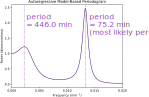
\includegraphics[width=\textwidth]{ar}
   \caption{
   }
   \label{fig:analysis-ar-periodogram}
  \end{subfigure}

  \caption{
    \textbf{(\ref{fig:analysis-ar-timeseries})}
    Sample time series (dark solid line), with a fitted autoregressive model (light solid line) of order 4 computed according to \textcite{jiaFrequencyDomainAnalysis2020}.
    \textbf{(\ref{fig:analysis-ar-periodogram})}
    Periodogram defined based on parameters of the autoregressive model.
    % The presence of a peak of height greater than 1 indicates that the time series is oscillatory.
    % Furthermore, the locations of peaks estimate the period of oscillation in the original time series.
  }
  \label{fig:analysis-ar}
\end{figure}

Fig.\ \ref{fig:analysis-ar} shows that the autoregressive model was able to correctly identify a time series as oscillatory, as evidenced by a peak in the periodogram of height greater than 1.
In addition, the periodogram correctly identifies a period of \SI{75.2}{\minute}.
However, when extended across a dataset of time series, very few time series within a dataset were classified as oscillatory using this method.
Unlike the classifier based on \textcite{glynnDetectingPeriodicPatterns2006a}, the autoregressive model does not having a parameter that can be adjusted to change the expected proportion of a dataset to be classified as oscillatory --- in other words, the tolerance of detecting rhythmicity cannot be adjusted.
Alternatively, the order of the model can be treated as a parameter, and model selection can be performed.
Nevertheless, among the time series that the algorithm classifies as oscillatory, the algorithm accurately estimates the frequency of oscillations.
%[Need: figures to summarise my investigation on population.  Probably need to re-do this on some datasets because it is poorly documented in my notes.]


\subsection{Machine learning approaches to classification}
\label{subsec:analysis-classification-ml}
% - Write results from classifier project (SVM, RF, etc.)


% [TODO] Worth re-doing the whole experiment using better data, e.g. the data I'm actually using in the biological results chapter.

As an alternative to the mathematical methods previously discussed, I trained a machine learning model --- specifically, a support vector classifier --- to classify oscillatory and non-oscillatory time series and identify features in the time series that discriminate between the two classes (appendix \ref{append:analysis-ml}).
%
% DESCRIPTION OF DATA
Specifically, I trained a support vector classifier on flavin time series from BY4741 cells  under \SI{10}{\gram~\litre^{-1}} glucose.
The dataset had 294 time series of 118 time points each.

% DATA PROCESSING

% [TODO] Repeat experiment with Butterworth filter, rather than sliding window detrending
To pre-process the data, I normalised each time series $x_{i} = x_{i,1}, x_{i,2}, \ldots , x_{i,j}, \ldots x_{i,n}$ by normalising it to produce a processed time series $z_{i} = z_{i,1}, z_{i,2}, \ldots , z_{i,j}, \ldots z_{i,n}$ as follows:

\begin{equation}
  z_{i,j} = \frac{x_{i,j} - \mu_{i}}{\sigma_{i}}
  \label{eq:analysis-stdscore}
\end{equation}

where $\mu_{i}$ is the mean value of $x_{i}$, and $\sigma_{i}$ is the standard deviation of $x_{i}$.
As a result, each normalised time series $z_{i}$ has a mean of 0 and a standard deviation of 1.

% LABELLING
Based on the normalised time series, I labelled them as non-oscillatory ($n_{0}=211$) and oscillatory ($n_{1}=83$).
% SPLITTING
From this input data, 150 time series formed the training set.

% FEATURISATION
% MODELS
\begin{figure}
  \centering
  \includegraphics[width=0.9\textwidth]{precision_recall}
  \caption[
  ]{
    (Left) Precision and (right) recall from five-fold cross-validation of support vector classifiers trained using different featurisation methods:
    (orange) using the time points as features,
    (green) using the power values in the Fourier spectrum as features,
    and (red) using \emph{catch22} features.
    (Blue) `random' indicates assigning time series to the oscillatory and non-oscillatory categories and used their time points as features, as a control.
  }
  \label{fig:analysis-precision-recall}
\end{figure}

% Replace with recursive feature elimination?
% This will modify the discussion paragraph below.
\begin{figure}
  \centering
  \includegraphics[width=0.5\textwidth]{catch22_training_featurevector_mean}
  \caption[
    Mean values of each \texttt{catch22} feature across each cell
  ]{
    Mean values of each \texttt{catch22} feature across each cell classified as non-oscillatory (class 0) or oscillatory (class 1) by an SVC from the testing set.
    The horizontal axis shows each \texttt{catch22} feature from 0 to 21, and the vertical axis shows the mean value of each feature across cells within an identified class.
  }
  \label{fig:analysis-svc-catch22}
\end{figure}

To determine the most effective way to featurise the data, I computed the precision and recall of support vector classifiers trained on data featurised using different methods.
Precision and recall were chosen as evaluation metrics due to the class imbalance, and the support vector classifiers were trained using a radial bias kernel, a kernel coefficient $\gamma = 1/N$, where $N$ is the number of features, and a regularisation parameter $C = 1$.

Fig.\ \ref{fig:analysis-precision-recall} suggests that featurisation using \textit{catch22} gave the best performance.
%[CONFIRM IMPORTANCE VIA RECURSIVE FEATURE ELIMINATION, USING RANDOM FOREST?]
Furthermore, Fig.\ \ref{fig:analysis-svc-catch22} suggests that the \texttt{FC\_LocalSimple\_mean3\_stderr} feature (represented as feature 9) is important for the classifier.
% Equation?
This feature is defined as the error based on using the mean of the previous three time points to predict each time point in the time series; time series that are more predictable should have low values of this feature.
Therefore, it is reasonable that oscillatory time series have higher values of this feature --- at any given time in the time series, the value changes substantially after three time points.
This is in contrast to noisy, non-oscillatory time series.

% ADAPTATION OF SVM: PREDICT PROBABILITIES

% Include result from randomly assigning labels as a control?
% This should give a `hill' in the middle.
\begin{figure}
  \centering
  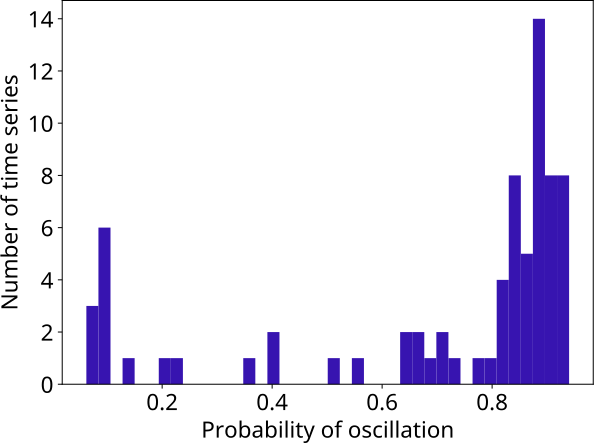
\includegraphics[width=0.5\textwidth]{classifier_histogram_probabilities_adapted}
  \caption{
    Histogram of probabilities of whether a time series in the test data set is classified as oscillatory by the SVC.
  }
  \label{fig:analysis-svc-proba-histogram}
\end{figure}


\begin{figure}
  \centering
  \begin{subfigure}[t]{0.45\textwidth}
  \centering
    \includegraphics[width=\linewidth]{proba_00}
    \caption{
    }
    \label{fig:analysis-svc-proba-00}
  \end{subfigure}%
  \begin{subfigure}[t]{0.45\textwidth}
  \centering
    \includegraphics[width=\linewidth]{proba_21}
    \caption{
    }
    \label{fig:analysis-svc-proba-21}
  \end{subfigure}

  \begin{subfigure}[t]{0.45\textwidth}
  \centering
    \includegraphics[width=\linewidth]{proba_38}
    \caption{
    }
    \label{fig:analysis-svc-proba-38}
  \end{subfigure}%
  \begin{subfigure}[t]{0.45\textwidth}
  \centering
    \includegraphics[width=\linewidth]{proba_61}
    \caption{
    }
    \label{fig:analysis-svc-proba-61}
  \end{subfigure}

  \begin{subfigure}[t]{0.45\textwidth}
  \centering
    \includegraphics[width=\linewidth]{proba_88}
    \caption{
    }
    \label{fig:analysis-svc-proba-88}
  \end{subfigure}%
  \begin{subfigure}[t]{0.45\textwidth}
  \centering
    \includegraphics[width=\linewidth]{proba_99}
    \caption{
    }
    \label{fig:analysis-svc-proba-99}
  \end{subfigure}
  \caption{
    Sample test set time series arranged by probability that each is oscillatory, as predicted by the support vector classifier:
    \textbf{(\ref{fig:analysis-svc-proba-00})} 0\%,
    \textbf{(\ref{fig:analysis-svc-proba-21})} 21\%,
    \textbf{(\ref{fig:analysis-svc-proba-38})} 38\%,
    \textbf{(\ref{fig:analysis-svc-proba-61})} 61\%,
    \textbf{(\ref{fig:analysis-svc-proba-88})} 88\%,
    \textbf{(\ref{fig:analysis-svc-proba-99})} 99\%,
  }
  \label{fig:analysis-svc-proba-gallery}
\end{figure}

To predict the probability that each time series is oscillatory to account for uncertainties, in contrast to assigning each test time series to one of two categories, I extended the support vector classifier to predict probabilities.
This was performed using Platt scaling \parencite{plattProbabilisticOutputsSupport1999}, as implemented by \texttt{scikit-learn}.
Fig.\ \ref{fig:analysis-svc-proba-histogram} shows that the distribution of probabilities falls in a U-shape.
This distribution is desirable because it indicates that the classifier is for the most part `certain' whether a time series is oscillatory.
In addition, these probabilities can also serve as a score for the quality of oscillations, as illustrated by Fig.\ \ref{fig:analysis-svc-proba-gallery}.

%[MORE EVALUATION? e.g. ROC curve, precision-recall curve.  MAYBE IT IS OVERKILL HERE.]

In sum,
a simple machine learning architecture is sufficient in classifying noisy biological time series into oscillatory and non-oscillatory categories, complete with probabilities.
This method was also able to identify which time series feature was the most important in distinguishing between oscillatory and non-oscillatory time series.


\section[Characterisation]{Characterisation: I have one time series --- what properties does it have?}
\label{sec:analysis-characterisation}

Characterising features of oscillatory time series is important as it provides a quantitative measure of how yeast metabolic cycles respond to genetic nutrient perturbations.
The characteristics that are important to my investigation of the yeast metabolic cycle include the period and the amplitude.
The period of an oscillatory time series is the easiest characteristic to compute a fixed number for because it is well-defined.
Similarly, the amplitude is easy to estimate, based on fitting a cosine to the signal, but are inadequate if oscillations are asymmetrical.
However, due to the detrending methods I used, information about the amplitude is lost, and therefore it must be indirectly inferred from the magnitude of noise, assuming that the sources of noise are constant across time series.


\subsection{Autocorrelation function}
\label{subsec:analysis-characterisation-acf}

In this section, I show that the autocorrelation function can be adapted to characterise the period and noise properties of populations of both sinusoid time series and time series and asymmetrical oscillations.
I first do so with synthetic time series with known properties and adapt the methods to my data that exhibit similar oscillations as the synthetic time series.

\subsubsection{Mathematical definitions}
\label{subsubsec:analysis-characterisation-acf-maths}

The cross-correlation function used in this chapter is adapted from \textcite{pietschDeterminingGrowthRates2023}, as follows:

\begin{enumerate}
  \item Let the data have $M$ cells.
        Each cell $i$ in the population of $M$ cells has a time series $x_{1}^{(i)}, \ldots , x_{j}^{(i)}, \ldots , x_{N}^{(i)}$ of quantity $x$ and a time series $y_{1}^{(i)}, \ldots , y_{j}^{(i)}, \ldots , y_{N}^{(i)}$ of quantity $y$.
        Let both time series have a sampling interval of $\Delta t$.
  \item The deviation from the population mean for each time series is computed.
        This population mean is calculated over replicates at each time point.
        The caveat of this calculation is that the signals \emph{must} be out-of-phase, and I ensure this by generating synthetic signals with a random phase.
        Otherwise, the underlying signal will be subtracted from all time series and the cross-correlation of noise will be computed --- this is undesired.
        \begin{equation}
          \delta x_{t}^{(i)} = x_{t}^{(i)} - \frac{1}{M} \sum_{j}x_{t}^{(j)}
          \label{eq:xcf-dmeans-x}
        \end{equation}
        \begin{equation}
          \delta y_{t}^{(i)} = y_{t}^{(i)} - \frac{1}{M} \sum_{j}y_{t}^{(j)}
          \label{eq:xcf-dmeans-y}
        \end{equation}
  \item Based on \textcite{kivietStochasticityMetabolismGrowth2014}, the cross-covariance of the two time series $x$ and $y$ at a time lag of $r\Delta t$, is thus given by:
        \begin{equation}
          C_{xy}^{(i)}(r\Delta t) =
          \begin{cases}
            \frac{1}{N-r} \sum_{t=1}^{N-r} \delta x_{t}^{(i)} \cdot \delta y_{t+r}^{(i)} & \text{if } r \geq 0 \\
            C_{yx}^{(i)}(-r \Delta t) & \text{if } r < 0
          \end{cases}
          \label{eq:xcf-xcov}
        \end{equation}
    \item $C_{xx}^{(i)}(0)$ and $C_{yy}^{(i)}(0)$ thus give the variances of $x$ and $y$.  The cross-correlation is thus given, with normalising by the standard deviation, by:
        \begin{equation}
          R_{xy}^{(i)}(r \Delta t) = \frac{C_{xy}^{(i)}(r \Delta t)}{\sqrt{C_{xx}^{(i)}(0) C_{yy}^{(i)}(0)}}
          \label{eq:xcf-xcf}
        \end{equation}
\end{enumerate}

The autocorrelation of a time series $x$ is thus the cross-correlation of the time series with itself, i.e.\ $R_{xx}^{(i)}(r \Delta t)$.


To understand the effect of the autocorrelation function on biological time series, I modelled time series flavin fluorescence oscillations using the harmonic oscillator and modelled time series of histone 2B abundance patterns using the FitzHugh-Nagumo oscillator \parencite{fitzhughImpulsesPhysiologicalStates1961}.
These model oscillators are defined by simple differential equations and are well-characterised.

The harmonic oscillator $y(t)$ is defined as the solution of:

\begin{equation}
  \sndif{y}{t} = -\omega^{2}y
  \label{eq:harmonic}
\end{equation}

where the sole parameter $\omega$ represents the angular frequency.
%The solution $y(t) = A \sin(\omega{}t + \phi)$ defines a sinusoidal time series; $A$ is a constant representing amplitude and $\phi$ is a constant representing phase, both determined by initial conditions of the system.


\begin{figure}
  \centering
  \includegraphics[width=0.9\linewidth]{fitzhughnagumo_sample.png}
  \caption[
    Sample time series based on the solution of the FitzHugh-Nagumo model
  ]
  {
    Sample time series based on the solution $v(t)$ of the FitzHugh-Nagumo model, with parameters
    $RI_{\mathrm{ext}}$ = 0.4, $\tau$ = 12.5, $a$ = 0.7, $b$ = 0.82.
  }
  \label{fig:fitzhughnagumo_sample}
\end{figure}

The FitzHugh-Nagumo oscillator $v(t)$ is defined as a solution of the system:

\begin{equation}
  \begin{aligned}
    \ndif{v}{t} &= v - \frac{v^3}{3} - w + RI_{\mathrm{ext}} \\
    \tau \ndif{w}{t} &= v + a - bw
  \end{aligned}
  \label{eq:fhn}
\end{equation}

where $RI_{\mathrm{ext}}$, $\tau$, $a$, and $b$ are constant parameters to be determined.
Fig.\ \ref{fig:fitzhughnagumo_sample} shows an example.


Biological time series have noise.
To assess the affect of noise on the cross-correlation function, I added Gaussian or Gillespie noise to the models of oscillators.

Gaussian noise was generated by randomly drawing samples from the normal distribution $\mathcal{N}(0,\sigma^{2})$.
Here, $\sigma$ denotes the standard deviation of the distribution and thus controls the size of the noise.


\begin{figure}
  \centering
  \begin{subfigure}{0.4\textwidth}
    \centering
    % Modify this figure:
    % - Axis labels
    \includegraphics[width=\linewidth]{gillespie}
    \caption{
    }
    \label{fig:gillespie_trajectory}
  \end{subfigure}%
 \begin{subfigure}{0.6\textwidth}
    \centering
    \includegraphics[width=\linewidth]{gillespie_noise_samples}
    \caption{
    }
    \label{fig:gillespie_noise_samples}
  \end{subfigure}

  \caption{
    \textbf{(\ref{fig:gillespie_trajectory})}
    Sample trajectory of a substrate created and destroyed by the birth-death process, simulated by the Gillespie algorithm ($k_{0} = 5$, $d_{0} = 0.05$, $t_{\mathrm{max}} = 1500$).
    \textbf{(\ref{fig:gillespie_noise_samples})}
    Sample time series of Gillespie noise, derived from trajectories generated as in (\ref{fig:gillespie_trajectory}).
  }
  \label{fig:gillespie_noise}
\end{figure}

Gillespie noise emulates noise from biological systems (Fig.\ \ref{fig:gillespie_noise}).
Gillespie noise was generated using the direct method of the Gillespie algorithm \parencite{gillespieExactStochasticSimulation1977} on the birth-death process model (appendix~\ref{append:analysis-gillespie}).
The parameters of the birth-death process control noise parameters.
Specifically, given a birth rate $k_{0}$ and a death rate $d_{0}$, the noise has a standard deviation of noise amplitude $A = \sqrt{k_{0}/d_{0}}$ and noise timescale $\tau = 1/d_{0}$.


\subsubsection{Effect of noise parameters on the autocorrelation function}
\label{subsubsec:analysis-characterisation-acf-sinusoid}

\begin{figure}
  \centering
  \begin{subfigure}[t]{0.45\textwidth}
  \centering
  % TODO: Replace with 3 sinusoids
    \includegraphics[width=\linewidth]{sinusoids_outofphase}
    \caption{
    }
    \label{fig:acf-sinusoids-nonoise-ts}
  \end{subfigure}%
  \centering
  \begin{subfigure}[t]{0.4\textwidth}
  \centering
    \includegraphics[width=\linewidth]{sinusoids_outofphase_acf_corrected}
    \caption{
    }
    \label{fig:acf-sinusoids-nonoise-acf}
  \end{subfigure}

  % TODO: Use the (high) noise level quoted, and generate 3 sinusoids to replace this,
  % as above.
  \begin{subfigure}[t]{0.45\textwidth}
  \centering
    \includegraphics[width=\linewidth]{noisysinusoids_outofphase}
    \caption{
    }
    \label{fig:acf-sinusoids-gausnoise-ts}
  \end{subfigure}%
  \centering
  \begin{subfigure}[t]{0.4\textwidth}
  \centering
    \includegraphics[width=\linewidth]{verynoisysinusoids_outofphase_acf}
    \caption{
    }
    \label{fig:acf-sinusoids-gausnoise-acf}
  \end{subfigure}

  \begin{subfigure}[t]{0.6\textwidth}
  \centering
    \includegraphics[width=\linewidth]{gillespie_k5_d0p05_mean}
    \caption{
    }
    \label{fig:acf-sinusoids-gillnoise-ts}
  \end{subfigure}%
  \centering
  \begin{subfigure}[t]{0.4\textwidth}
  \centering
    \includegraphics[width=\linewidth]{gillespie_k5_d0p05_acf}
    \caption{
    }
    \label{fig:acf-sinusoids-gillnoise-acf}
  \end{subfigure}

  \caption{
    %Effect of type of noise on the autocorrelation function.
    \textbf{(\ref{fig:acf-sinusoids-nonoise-ts})} Sample sinusoids without noise, and 
    \textbf{(\ref{fig:acf-sinusoids-nonoise-acf})} its autocorrelation function.
    %
    \textbf{(\ref{fig:acf-sinusoids-gausnoise-ts})} Sample sinusoids with Gaussian noise defined by drawing samples from $\mathcal{N}(0,\sigma^{2}=3)$, and 
    \textbf{(\ref{fig:acf-sinusoids-gausnoise-acf})} its autocorrelation function.
    %
    \textbf{(\ref{fig:acf-sinusoids-gillnoise-ts})} Sample sinusoids of with Gillespie noise ($k_{0} = 5$ and $d_{0} = 0.05$), and 
    \textbf{(\ref{fig:acf-sinusoids-gillnoise-acf})} its autocorrelation function.
    Red line is defined by $y = \me^{-2d_{0}T}$, where $T$ represents the lag in units of period of the sinusoids.
    %
    For each case, the frequency of the sinusoids was 0.03, and there were 100 repeats, randomly out-of-phase.
  }
  \label{fig:acf-sinusoids}
\end{figure}

To compare the effect of Gaussian noise and Gillespie noise on the autocorrelation function, I computed the population autocorrelation from a population of sinusoids augmented with the two types of noise.

% [Show working -- i.e. the mathematical derivations that make me expect results?]
% [Equations -- clear lines before/after, rather than having them in-line?]

Fig.\ \ref{fig:acf-sinusoids-nonoise-acf} shows that the autocorrelation function computed from a population of out-of-phase sinusoids can be modelled by the function $y(T) = cos(2 \pi T)$, where $f$ is the frequency of the sinusoids and $T$ is the lag in units of the periods of the sinusoid.
This relationship can be confirmed by deriving from the definition of the autocorrelation function used in this chapter (mathematical derivation in appendix ...).

Following this, Fig.\ \ref{fig:acf-sinusoids-gausnoise-acf} shows that the addition of Gaussian noise preserved the point $y(0) = 1$, but the amplitude of the cosine that models the autocorrelation function is reduced.
Furthermore, the variation of the autocorrelation function among time series at long lags is increased, evidenced by the interquartile range.
This variation is because less data was used to compute the autocorrelation function at long lags (mathematical derivation in appendix ...).

% [Show working -- i.e. the mathematical derivations that make me expect this exponential fit?]
% Though Peter said this `is not trivial'.
Fig.\ \ref{fig:acf-sinusoids-gillnoise-acf} then shows that when Gillespie noise was added to the sinusoids, the medium autocorrelation followed the exponential decay function $y = \me^{-2d_{0}T}$, where $T$ represents lag.
In addition, the location of the peaks --- corresponding to the period of the sinusoid --- were preserved.
This figure thus suggests that the death rate $d_{0}$ parameter of Gillespie noise controlled the shape of the autocorrelation function.


\begin{figure}
  \centering
  \begin{subfigure}[t]{0.6\textwidth}
  \centering
    \includegraphics[width=\linewidth]{gillespie_k5_d0p5_mean.png}
    \caption{
    }
    \label{fig:acf-noisetimescale-highd0-ts}
  \end{subfigure}%
  \begin{subfigure}[t]{0.4\textwidth}
  \centering
    \includegraphics[width=\linewidth]{gillespie_k5_d0p5_acf.png}
    \caption{
    }
    \label{fig:acf-noisetimescale-highd0-acf}
  \end{subfigure}

  \begin{subfigure}[t]{0.6\textwidth}
  \centering
    \includegraphics[width=\linewidth]{gillespie_k5_d0p005_mean.png}
    \caption{
    }
    \label{fig:acf-noisetimescale-lowd0-ts}
  \end{subfigure}%
  \begin{subfigure}[t]{0.4\textwidth}
  \centering
    \includegraphics[width=\linewidth]{gillespie_k5_d0p005_acf.png}
    \caption{
    }
    \label{fig:acf-noisetimescale-lowd0-acf}
  \end{subfigure}

  \caption[
    Effect of death rate of Gillespie noise on the autocorrelation function.
  ]{
    %Effect of death rate ($d_{0}$) of Gillespie noise on the autocorrelation function.
    \textbf{(\ref{fig:acf-noisetimescale-highd0-ts})} Sample sinusoids with Gillespie noise ($k_{0} = 5$ and $d_{0} = 0.5$), and 
    \textbf{(\ref{fig:acf-noisetimescale-highd0-acf})} its autocorrelation function.
    %
    \textbf{(\ref{fig:acf-noisetimescale-lowd0-ts})} Sample sinusoids with Gillespie noise ($k_{0} = 5$ and $d_{0} = 0.005$), and 
    \textbf{(\ref{fig:acf-noisetimescale-lowd0-acf})} its autocorrelation function.
    %
    Red lines are defined by $y = \me^{-2d_{0}T}$, where $T$ represents the lag in units of period of the sinusoids.
    %
    For each case, the frequency of the sinusoids was 0.03, and there were 100 repeats, randomly out-of-phase.
  }
  \label{fig:acf-noisetimescale}
\end{figure}


\begin{figure}
  \centering
  \begin{subfigure}[t]{0.5\textwidth}
  \centering
    \includegraphics[width=\linewidth]{acf_fit_example.png}
    \caption{
    }
    \label{fig:acf-noisetimescale-effect-fit}
  \end{subfigure}%
  \begin{subfigure}[t]{0.5\textwidth}
  \centering
    \includegraphics[width=\linewidth]{deathrate_vs_decay.png}
    \caption{
    }
    \label{fig:acf-noisetimescale-effect-relationship}
  \end{subfigure}

  \caption{
    %Characterising the autocorrelation function to quantify the effect of Gillespie noise timescale.
    \textbf{(\ref{fig:acf-noisetimescale-effect-fit})} Fitting exponential decay functions to estimate $d_{0}$ from the autocorrelation function.
    \textbf{(\ref{fig:acf-noisetimescale-effect-relationship})} The relationship between $d_{0}$ and the decay rate $D$ found from fitting exponential decay functions to the mean autocorrelation function, the peaks, and the troughs of this mean function.
    Here, $k_{0}$ was held constant at 5.
  }
  \label{fig:acf-noisetimescale-effect}
\end{figure}

To quantify the effect of the timescale of noise, defined by $\tau = 1/d_{0}$, I varied the death rate parameter $d_{0}$ when generating Gillespie noise that was to be added to the sinusoids.

Fig.\ \ref{fig:acf-noisetimescale} shows that a higher death rate decreased the decay timescale of the autocorrelation function (Fig.\ \ref{fig:acf-noisetimescale-highd0-ts}), while a lower death rate introduced long-term trends in the simulated signals (Fig.\ \ref{fig:acf-noisetimescale-highd0-ts}).
A lower death rate also increased the decay timescale for the autocorrelation function and increased the variation between autocorrelation functions between replicates (Fig.\ \ref{fig:acf-noisetimescale-lowd0-acf}).

To show how $d_{0}$ can be estimated from the autocorrelation function, I fit exponential decay functions of the form $y = (1-C)\me^{-DT}+C$ to the mean autocorrelation, the peaks of the mean function, and the troughs of the mean functions using non-linear least squares fitting, defining $C$ and $D$ as variable parameters (Fig.\ \ref{fig:acf-noisetimescale-effect-fit}).
Subsequently, Fig.\ \ref{fig:acf-noisetimescale-effect-relationship} suggests that the decay rates $D$ of the autocorrelation function indeed increases linearly with $d_{0}$
In other words, the death rate $d_{0}$ controls the decay rate $D$ of the autocorrelation function.
Conversely, if $D$ can be estimated from the autocorrelation function, then the noise timescale $\tau$ of the time series can be estimated.


\begin{figure}
  \centering
  \begin{subfigure}[t]{0.6\textwidth}
  \centering
    \includegraphics[width=\linewidth]{gillespie_k25_d0p05_mean.png}
    \caption{
    }
    \label{fig:acf-noiseamplitude-highk0-ts}
  \end{subfigure}%
  \begin{subfigure}[t]{0.4\textwidth}
  \centering
    \includegraphics[width=\linewidth]{gillespie_k25_d0p05_acf.png}
    \caption{
    }
    \label{fig:acf-noiseamplitude-highk0-acf}
  \end{subfigure}

  \begin{subfigure}[t]{0.6\textwidth}
  \centering
    \includegraphics[width=\linewidth]{gillespie_k1_d0p05_mean.png}
    \caption{
    }
    \label{fig:acf-noiseamplitude-lowk0-ts}
  \end{subfigure}%
  \begin{subfigure}[t]{0.4\textwidth}
  \centering
    \includegraphics[width=\linewidth]{gillespie_k1_d0p05_acf.png}
    \caption{
    }
    \label{fig:acf-noiseamplitude-lowk0-acf}
  \end{subfigure}

  \caption[
    Effect of birth rate of Gillespie noise on the autocorrelation function.
  ]{
    %Effect of birth rate ($k_{0}$) of Gillespie noise on the autocorrelation function.
    \textbf{(\ref{fig:acf-noiseamplitude-highk0-ts})} Sample sinusoids with Gillespie noise ($k_{0} = 25$ and $d_{0} = 0.05$), and 
    \textbf{(\ref{fig:acf-noiseamplitude-highk0-acf})} its autocorrelation function.
    %
    \textbf{(\ref{fig:acf-noiseamplitude-lowk0-ts})} Sample sinusoids with Gillespie noise ($k_{0} = 1$ and $d_{0} = 0.05$), and 
    \textbf{(\ref{fig:acf-noiseamplitude-lowk0-acf})} its autocorrelation function.
    %
    Red lines are defined by $y = \me^{-2d_{0}T}$, where $T$ represents the lag in units of period of the sinusoids.
    %
    For each case, the frequency of the sinusoids was 0.03, and there were 100 repeats, randomly out-of-phase.
  }
  \label{fig:acf-noiseamplitude}
\end{figure}


\begin{figure}
  \centering
  \includegraphics[width=0.6\linewidth]{birthrate_vs_ydispl.png}
  \caption[
    Quantifying the effect of Gillespie noise amplitude on the autocorrelation function
  ]{
    The relationship between the noise amplitude and the $y$-displacement $C$ found from fitting exponential decay functions to the mean autocorrelation function, the peaks, and the troughs of this mean function.
    Here, $d_{0}$ was held constant at 0.05.
  }
  \label{fig:acf-noiseamplitude-effect}
\end{figure}


To quantify the effect of the noise amplitude, defined by $A = \sqrt{k_{0}/d_{0}}$, I varied the birth rate parameter $k_{0}$ when generating Gillespie noise that was to be added to the sinusoids (Fig.\ \ref{fig:acf-noiseamplitude}).

Fig.\ \ref{fig:acf-noiseamplitude} shows that a lower birth rate decreased the amplitude of noise (Fig.\ \ref{fig:acf-noiseamplitude-lowk0-ts}) and decreased the variation between replicate autocorrelation functions (Fig.\ \ref{fig:acf-noiseamplitude-lowk0-acf}).
Conversely, a higher birth rate increased the amplitude of noise (Fig.\ \ref{fig:acf-noiseamplitude-highk0-ts}) and increased the variation between replicate autocorrelation functions (Fig.\ \ref{fig:acf-noiseamplitude-highk0-acf}).

To show how the noise amplitude can be estimated from the autocorrelation function, I fit exponential decay functions as in Fig.\ \ref{fig:acf-noisetimescale-effect-fit}.
Fig.\ \ref{fig:acf-noiseamplitude-effect} suggests that the $y$-displacements $C$ of the exponential fits to peaks and troughs converged to 0 as $k_{0}/d_{0}$ increased, showing that the amplitude of the oscillations in the autocorrelation function decreases as the noise amplitude increases.
In other words, the birth rate $d_{0}$ controls the $y$-displacement parameter $C$ of the autocorrelation function, which is a proxy for the function's amplitude.
Conversely, if $C$ can be estimated from the autocorrelation function, then the noise amplitude $A$ of the time series can be estimated.

% [Move to conclusion?]
% To conclude, if a population of replicate oscillatory time series is modelled with the sum of sinusoids and Gillespie noise, then the birth rate and death rate can control the shape of the autocorrelation function.
% The death rate controls the timescale of noise and thus how fast the autocorrelation decays as lag increases.
% The birth rate controls the amplitude of noise and thus controls how robust the autocorrelation function is.


\begin{figure}
  \centering
  \begin{subfigure}[t]{0.6\textwidth}
  \centering
    \includegraphics[width=\linewidth]{26643_ts.png}
    \caption{
    }
    \label{fig:acf-sinusoid-biol-ts}
  \end{subfigure}%
  \begin{subfigure}[t]{0.4\textwidth}
  \centering
    \includegraphics[width=\linewidth]{fy4_26643_plots_06.png}
    \caption{
    }
    \label{fig:acf-sinusoid-biol-acf}
  \end{subfigure}

  \caption{
    \textbf{(\ref{fig:acf-sinusoid-biol-ts})}
    Sample time series of flavin autofluorescence.
    \textbf{(\ref{fig:acf-sinusoid-biol-acf})}
    Autocorrelation function across a population of time series of flavin autofluorescence.
  }
  \label{fig:acf-sinusoid-biol}
\end{figure}

From the relationships shown in Figs.\ \ref{fig:acf-noiseamplitude-effect} and \ref{fig:acf-noisetimescale-effect}, noise parameters from the autocorrelation functions of real signals may be deduced.
Fig.\ \ref{fig:acf-sinusoid-biol} shows ...(INSERT RESULT OF NEW INVESTIGATION HERE).


\subsubsection{The autocorrelation function extended for use with FitzHugh-Nagumo oscillators}
\label{subsubsec:analysis-characterisation-acf-fhn}


\begin{figure}
  \centering
  \begin{subfigure}[t]{0.6\textwidth}
  \centering
    \includegraphics[width=\linewidth]{fhn_meanplot}
    \caption{
    }
    \label{fig:acf-fhn-gillnoise-ts}
  \end{subfigure}%
  \begin{subfigure}[t]{0.4\textwidth}
  \centering
    \includegraphics[width=\linewidth]{fhn_acf}
    \caption{
    }
    \label{fig:acf-fhn-gillnoise-acf}
  \end{subfigure}

  \caption{
    %The autocorrelation function of FitzHugh-Nagumo oscillators with Gillespie noise.
    \textbf{(\ref{fig:acf-fhn-gillnoise-ts})} Sample FitzHugh-Nagumo oscillators ($RI_{\mathrm{ext}}$ = 0.4, $\tau$ = 12.5, $a$ = 0.7, $b$ = 0.82) with Gillespie noise ($k_{0} = 5$ and $d_{0} = 0.05$), and 
    \textbf{(\ref{fig:acf-fhn-gillnoise-acf})} its autocorrelation function.
    Red line is defined by $y = \me^{-2d_{0}T}$, where $T$ represents the lag in units of period of the sinusoids.
    %
    There were 100 repeats, randomly out-of-phase.
  }
  \label{fig:acf-fhn}
\end{figure}


\begin{figure}
  \centering
  \begin{subfigure}[t]{0.45\textwidth}
  \centering
    \includegraphics[width=\linewidth]{fhn_expofit}
    \caption{
    }
    \label{fig:acf-fhn-noiseparams-fit}
  \end{subfigure}%
  \begin{subfigure}[t]{0.45\textwidth}
  \centering
    \includegraphics[width=\linewidth]{fhn_highnts_expofit}
    \caption{
    }
    \label{fig:acf-fhn-noiseparams-fit-highnts}
  \end{subfigure}

  \begin{subfigure}[t]{0.45\textwidth}
  \centering
    \includegraphics[width=\linewidth]{fhn_deathrate_vs_decay.png}
    \caption{
    }
    \label{fig:acf-fhn-noiseparams-noisetimescale}
  \end{subfigure}%
  \begin{subfigure}[t]{0.45\textwidth}
  \centering
    \includegraphics[width=\linewidth]{fhn_birthrate_vs_ydispl.png}
    \caption{
    }
    \label{fig:acf-fhn-noiseparams-noiseamplitude}
  \end{subfigure}

  \caption{
    %Quantifying the effect of Gillespie noise parameters on the autocorrelation function of FitzHugh-Nagumo oscillators.
    \textbf{(\ref{fig:acf-fhn-noiseparams-fit})}
    Fitting exponential decay functions of the form $y = (1-C)\me^{-DT}+C$, with $C$ and $D$ as variable parameters, to the autocorrelation function, generated with $k_{0}=5$ and $d_{0}=0.05$, and
    \textbf{(\ref{fig:acf-fhn-noiseparams-fit-highnts})}
    with $k_{0}=5$ and $d_{0}=0.005$.
    \textbf{(\ref{fig:acf-fhn-noiseparams-noisetimescale})}
    The relationship between $d_{0}$ and the decay rate $D$ ($k_{0}=5$).
    \textbf{(\ref{fig:acf-fhn-noiseparams-noiseamplitude})}
    The relationship between $k_{0}/d_{0}$ and $y$-displacement $C$ of the exponential fit ($d_{0}=0.05$)
  }
  \label{fig:acf-fhn-noiseparams}
\end{figure}

To test whether Gillespie noise parameters can be estimated from the autocorrelation function computed from oscillations of a different shape, I repeated the exponential fitting in section~\ref{subsubsec:analysis-characterisation-acf-sinusoid} on the FitzHugh-Nagumo oscillator.

Fig.\ \ref{fig:acf-fhn-gillnoise-acf} shows that when the oscillator had a different shape, the shape of the autocorrelation function changed: i.e.\ the waves in the autocorrelation function were more pointed.
In addition, fitting an exponential decay function to the autocorrelation function to estimate noise parameters was less reliable, particularly with high noise timescales (Fig.\ \ref{fig:acf-fhn-noiseparams-fit-highnts}).
As a consequence, estimating the noise timescale $\tau$ from the decay rate $D$ of the exponential decay function produced a greater range of uncertainty (Fig.\ \ref{fig:acf-fhn-noiseparams-noisetimescale}).
However, estimating the noise amplitude $A$ based on the y-displacement $C$ of the exponential decay function remained as reliable as the sinusoid oscillator case (Fig.\ \ref{fig:acf-fhn-noiseparams-noiseamplitude}).


\begin{figure}
  \centering
  \begin{subfigure}[t]{0.6\textwidth}
  \centering
  % TODO: Edit out the flavin bits
    \includegraphics[width=\linewidth]{htb2mCherry_26643_plots_purple_01.pdf}
    \caption{
    }
    \label{fig:acf-fhn-biol-ts}
  \end{subfigure}%
  \begin{subfigure}[t]{0.4\textwidth}
  \centering
    \includegraphics[width=\linewidth]{htb2mCherry_26643_plots_mCh_06.png}
    \caption{
    }
    \label{fig:acf-fhn-biol-acf}
  \end{subfigure}

  \caption{
    \textbf{(\ref{fig:acf-fhn-biol-ts})}
    Sample time series of histone 2B abundance (pink).
    \textbf{(\ref{fig:acf-fhn-biol-acf})}
    Autocorrelation function across a population of time series of histone 2B abundance.
  }
  \label{fig:acf-fhn-biol}
\end{figure}

From the relationships shown in Figs.\ \ref{fig:acf-fhn-noiseparams-noisetimescale} and \ref{fig:acf-fhn-noiseparams-noiseamplitude}, noise parameters from the autocorrelation functions of real signals may be deduced.
Fig.\ \ref{fig:acf-fhn-biol} shows ...(INSERT RESULT OF NEW INVESTIGATION HERE).

% Not sure how useful this subsection is...
% And it's also a bit dangling
\subsection{Combining methods to get a picture of periodicity}
\label{subsec:analysis-characterisation-combined}

\begin{figure}
  \centering
  \includegraphics[width=0.5\linewidth]{potvin-trottierSynchronousLongtermOscillations2016_1e_adapted}
  \caption[
    Autocorrelation function and power spectral density calculated time series of cellular YFP concentration
  ]{
    Autocorrelation function (main) and power spectral density (upper-right inset) calculated over \num{8694} cell divisions' worth of time series of cellular YFP concentration controlled by a YFP-expressing repressilator.
    From the autocorrelation function, the average period of the oscillations is 5.6 generations, and the peak frequency of the power spectral density agrees.
    Adapted from \textcite{potvin-trottierSynchronousLongtermOscillations2016}.
  }
  \label{fig:acf-fft-example}
\end{figure}

Each periodicity-estimation method has a limited ability to estimate the period of short, noisy biological time series; therefore, it is often useful to combine several such methods to produce a picture of the periodicity of oscillatory time series.
For example, \textcite{potvin-trottierSynchronousLongtermOscillations2016} combines the autocorrelation function and the Fourier transform to study the changes in the periodicity of a modified model of the repressilator (Fig.\ \ref{fig:acf-fft-example}).
%Thus, in my subsequent analysis of biological data, I combine the autocorrelation function and the Fourier spectrum.

% [FIGURE: SHOWS A GOOD TIME SERIES, FFT, ACF, AR, AND THE MOST PROBABLY OSCILLATION FREQUENCY FROM EACH]

% [FIGURE: THE SAME AS ABOVE BUT LOOKING AT A POPULATION OF TIME SERIES.  THESE TRAJECTORIES SHOULD HAVE BEEN COMPUTED INDIVIDUALLY FOR EACH TIME SERIES.  THE CAPTION SHOULD EXPLAIN THE MEAN/MEDIAN AND ERROR RANGES.]

\subsection{New subsection for noise}
\label{subsec:analysis-characterisation-noise}

\begin{figure}
  \centering
  \begin{subfigure}[htpb]{0.5\textwidth}
   \centering
   \includegraphics[width=\textwidth]{snr_illustration}
   \caption{
   }
   \label{fig:analysis-snr-illustration}
 \end{subfigure}%
 \begin{subfigure}[htpb]{0.5\textwidth}
   \centering
   \includegraphics[width=\textwidth]{pyruvate_snr_edit}
   \caption{
   }
   \label{fig:analysis-snr-histogram-example}
  \end{subfigure}

  \caption{
    %The signal-to-noise ratio as a measure of signal quality.
    \textbf{(\ref{fig:analysis-snr-illustration})}
    Illustration of signal-to-noise ratio.
    The signal-to-noise ratio is defined (Eqs.\ \ref{eq:normalised-periodogram}--\ref{eq:noise}) as the area under the periodogram below a cut-off frequency (yellow) divided by the area under the periodogram above a cut-off frequency (pink).
    \textbf{(\ref{fig:analysis-snr-histogram-example})}
    Histogram of signal-to-noise ratios from a sample experiment ($n=403$).
  }
  \label{fig:analysis-snr}
\end{figure}

To evaluate the quality of oscillatory time series in a dataset and to indirectly measure the amplitude of the oscillations, I computed a signal-to-noise ratio for each time series.
Because the information about the amplitude of the oscillations was removed when they were filtered using the high-pass Butterworth filter, a different measure is needed.
Assuming a constant noise introduced by the combination of intrinsic noise (stochasticity in biochemical processes) and extrinsic noise (variations introduced by measurement instruments), a low signal-to-noise ratio suggests a low oscillation amplitude, and the reverse is true for a high signal-to-noise ratio.

The signal-to-noise ratio can be defined as follows:

Given a time series $x(t) = x_{t_{1}}, x_{t_{2}}, \ldots, x_{t_{N}}$, the normalised classical periodogram (Fourier spectrum) is given by

\begin{equation}
  P(\omega) = \frac{N}{2\sigma^{2}} \left|\int_{-\infty}^{\infty} x(t) e^{-2\pi it}dt \right|, % check constants, etc
  \label{eq:normalised-periodogram}
\end{equation}

where $N$ is the number of time points in $x$ and $\sigma^{2}$ is the sample variance of $x$.
The periodogram $P$ is defined as a function of the angular frequency $\omega$.

A critical frequency $\omega_{c}$ is then defined to divide signal and noise --- that is, very high-frequency components of the periodogram correspond to noise and lower-frequency components correspond to the meaningful oscillations.

The signal to noise ratio $r_{s/n}$ (Fig.\ \ref{fig:analysis-snr}) is thus defined as

\begin{equation}
  r_{s/n} = \frac{s}{n}
  \label{eq:snr}
\end{equation}

where the signal $s$ is defined as

\begin{equation}
  s = \int_{0}^{\omega_{c}} P(\omega) d\omega
  \label{eq:signal}
\end{equation}

and the noise $n$ is defined as

\begin{equation}
  n = \int_{\omega_{c}}^{\infty} P(\omega) d\omega
  \label{eq:noise}
\end{equation}

In this thesis, I define $\omega_{c} = \SI[parse-numbers=false]{1/350}{\minute^{-1}}$ because this frequency is lower than the frequencies of all oscillations of flavin autofluorescence I observed in my experiments.


\section[Correlation]{Correlation: I have two signals from the same cell --- what are their relationships to each other?}
\label{sec:analysis-correlation}

So far, I have considered one type of time series from the yeast metabolic oscillator at a time.
However, the yeast metabolic oscillator and the cell division cycle form part of a system of coupled oscillators
In my experiments I record signals that monitor both.
Investigating correlations between two paired time series, originating from the same cell, leads to an understanding of the relationship between the two oscillators.
The most important being the phase relationship: does one oscillation lag behind the other, to what extent, and is this consistent across cells?

% [COMMENTED OUT BECAUSE IT IS THE SOLE SUBSECTION]
% \subsection{Cross-correlation}
% \label{subsec:analysis-correlation-xcf}

In signal processing, cross-correlation is used to measure how similar two time series are, as the displacement of one relative to the other is shifted across the length of the time series.
In a biological context, cross-correlation has been used to investigate the relationship between the expression levels of two genes in a model feed-forward loop \parencite{dunlopRegulatoryActivityRevealed2008},
and to investigate the relationship between instantaneous growth rate and the expression of \textit{lac} genes OR of enzymes in central metabolism across a population of \textit{E. coli} cells \parencite{kivietStochasticityMetabolismGrowth2014}.
Importantly, \textcite{kivietStochasticityMetabolismGrowth2014} employs a single-cell microfluidics experiment with time-lapse microscopy, and therefore their treatment of a population of time series is useful for my case.
Therefore, my use of cross-correlation is adapted from theirs so that it suits a population of time series.
My implementation has already been described in section~\ref{subsubsec:analysis-characterisation-acf-maths}.

As in my discussion of autocorrelation (section~\ref{subsec:analysis-characterisation-acf}), I will start with the sinusoid and FitzHugh-Nagumo oscillators as simulations of my biological time series to show understanding of the methods, then apply the understand to a real dataset.

\begin{figure}
  \centering
  \begin{subfigure}[t]{0.45\textwidth}
  \centering
  % TODO: Squish so that it is consistent with adjacent figure
    \includegraphics[width=\linewidth]{sinusoid_and_fitzhughnagumo_nonoise.png}
    \caption{
      Sample FitzHugh-Nagumo oscillator (orange) generated with parameters $RI_{\mathrm{ext}}$ = 0.4, $\tau$ = 12.5, $a$ = 0.7, $b$ = 0.82, and a sinusoid of frequency 0.026 (blue), adjusted so that its frequency is the same as that of the FitzHugh-Nagumo oscillator.
    }
    \label{fig:xcf-nonoise-ts}
  \end{subfigure}%
  \centering
  \begin{subfigure}[t]{0.45\textwidth}
  \centering
    \includegraphics[width=\linewidth]{randomshift_sinusoid_fitzhughnagumo_xcf.png}
    \caption{
      Cross-correlation function of the FitzHugh-Nagumo oscillator with respect to the sinusoid oscillator, based on 400 pairs of signal as in~\ref{fig:xcf-nonoise-ts}, each pair randomly phase-shifted.
    }
    \label{fig:xcf-nonoise-xcf}
  \end{subfigure}

  % TODO: Use Gillespie noise.  Maybe this figure already exists.
  \begin{subfigure}[t]{0.45\textwidth}
  \centering
    \includegraphics[width=\linewidth]{sinusoid_and_fitzhughnagumo_gillnoise.png}
    \caption{
      FitzHugh-Nagumo (orange) and sinusoid oscillators (blue), as in~\ref{fig:xcf-nonoise-ts}, but with Gillepsie noise ($d_{0} = 0.05$, $k_{0} = 5$).
    }
    \label{fig:xcf-gillnoise-ts}
  \end{subfigure}%
  \centering
  \begin{subfigure}[t]{0.45\textwidth}
  \centering
    \includegraphics[width=\linewidth]{randomshift_sinusoid_fitzhughnagumo_gillnoise_xcf.png}
    \caption{
      Cross-correlation function of the FitzHugh-Nagumo oscillator with respect to the sinusoid oscillator, based on 400 pairs of signal as in~\ref{fig:xcf-gillnoise-ts}, each pair randomly phase-shifted.
    }
    \label{fig:xcf-gillnoise-xcf}
  \end{subfigure}

  \caption{
    Using the cross-correlation function to evaluate the shift of one synthetic time series relative to another with a different shape.
  }
  \label{fig:xcf}
\end{figure}

First, I generated a population of 400 FitzHugh-Nagumo oscillators and a population of 400 sinusoids so that they have the same period as the FitzHugh-Nagumo oscillator, but shifted in phase (figure~\ref{fig:xcf-nonoise-ts}).
This simulates flavin autofluorescence oscillations and oscillations in histone 2B abundance both being at the same frequency, owing to the coupling between the metabolic cycle and the cell division cycle, but may be out of phase.
The cross-correlation function of each FitzHugh-Nagumo oscillator with respect to the sinusoid oscillator, across the population, was computed (figure~\ref{fig:xcf-nonoise-xcf}).
If the two types of oscillators are in phase (i.e.\ the peaks coincide), the cross-correlation at lag 0 should be 1.
However, as the two oscillators are shifted in phase relative to each other, this peak of the cross-correlation function is shifted to the right, and the $x$-position of this peak thus indicates the average time by which the FitzHugh-Nagumo oscillator is shifted forward relative to the sinusoid oscillator, across the population.
As before, I added noise (figure~\ref{fig:xcf-gillnoise-ts}) to investigate the effect on the cross-correlation function (figure~\ref{fig:xcf-gillnoise-xcf}).
This illustrates that the cross-correlation function can still find phase relationships between two types of oscillatory data, even if the noise is extreme.

% TODO: Replace with pyruvate?  More dramatic.
\begin{figure}
  \centering
  \begin{subfigure}[t]{0.9\textwidth}
  \centering
    \includegraphics[width=\linewidth]{htb2mCherry_26643_plots_purple_01.pdf}
    \caption{
      Sample time series of flavin autofluorescence (purple) and histone 2B abundance (pink).
    }
    \label{fig:xcf-biol-ts}
  \end{subfigure}

  \begin{subfigure}[t]{0.7\textwidth}
  \centering
    \includegraphics[width=\linewidth]{xcf_edit.pdf}
    \caption{
      Cross-correlation function of the histone 2B abundance time series with respect to the flavin autofluorescence time series.
    }
    \label{fig:xcf-biol-xcf}
  \end{subfigure}

  \caption{
    Using the cross-correlation function to evaluate the shift of histone 2B abundance traces with respect to flavin autofluorescence traces.
  }
  \label{fig:xcf-biol}
\end{figure}

I can thus use this method to quantify the shift of the cell division cycle relative to the yeast metabolic cycle, therefore assessing the relationship between the two oscillators.
Figure~\ref{fig:xcf-biol} shows such as example, which demonstrates that the histone 2B oscillations succeed the flavin autofluorescence oscillations by an average of \SI{5}{\minute}.

% \subsection{Granger Causality}
% \label{sec:analysis-correlation-granger}

% Granger causality is another method of assessing the relationship between two time series.
% It is a statistical hypothesis test used to answer the question of whether one time series is useful for predicting another [CITATION FOR GRANGER CAUSALITY TEST NEEDED] -- in other words, it evaluates precedence of one time series relative to another.
% The logic of the Granger causality test is that: given a time series X and a time series Y, if you can predict values of Y based on the values of X better than you can predict values of Y based on the past values of Y, then X Granger-causes Y.
% This method is used a lot in econometrics and climate science [CITATIONS NEEDED].
% [AND DO BIOLOGISTS USE IT?]

% (Add content when I figure out how to make this investigation work.)

\section[Clustering]{Clustering: I have many time series (of the same signal) from many cells --- what are their relationships to each other?}
\label{sec:analysis-clustering}

% Literature review subsection
% \subsection{(Literature)}
% \label{subsec:analysis-clustering-literature}

% mini-review -- IT'S PRETTY UNWIELDY AT THIS POINT, AND REFERENCES CONCEPTS NOT DISCUSSED TILL LATER
Clustering of time series has been used to identify groupings within a set of time series \parencite{wangStructureBasedStatisticalFeatures2007}, including fMRI signals \parencite{shafieiDopamineSignalingModulates2019}, or even transcript cycling patterns in YMCs \parencite{tuLogicYeastMetabolic2005}.
However, \textcite{wangStructureBasedStatisticalFeatures2007} and \textcite{tuLogicYeastMetabolic2005} employed $k$-means clustering, which requires the user to specify the number of clusters, and therefore may not reflect the underlying structure of the set of time series.
Though \textcite{shafieiDopamineSignalingModulates2019} used modularity clustering \parencite{newmanModularityCommunityStructure2006}, their method was based on one time series feature, which may not adequately capture the characteristics of the time series.

Clustering is important because it can discover structure in a dataset and can summarise the difference between the groups it finds.
For my study of the yeast metabolic cycle, clustering would help address whether such differences conform to existing labels in the dataset, for example, cells grouped by strain or by nutrient condition.
It could then identify the time series features that are responsible for distinguishing between groups.
Furthermore, clustering is important for a dataset from which we expect cell-to-cell heterogeneity because it may discover subpopulations in the dataset.

The data for this section consists of flavin autofluorescence oscillation from one experiment with both BY4741 (background strain) and zwf1$\Delta$ (mutant strain) strains.
I expected the zwf1$\Delta$ traces to show different properties, as it is a strain that did not show oscillations in dissolved oxygen in the chemostat~\parencite{tuCyclicChangesMetabolic2007}.

% \subsection{Machine learning approaches to clustering}
% \label{subsec:analysis-clustering-ml}
% - Featurisation -- decisions to make
% - Clustering approaches and algorithms -- compare and contrast
% - Review existing methods first and then talk about the methods I tried, with results.

% Copied from 10m report.
% - Supervised classification is going to be mostly killed because it belongs in a previous section, and I have better data than SM vs SC.
% - Unsupervised clustering: the literature stays, but I'll try doing it on better data.  To add: UMAP.
% ----------------------
\subsection{Graph-based clustering}
\label{subsec:analysis-clustering-graphclustering}

% FIGURE: pipeline and options.  It's rather difficult to visualise what happens, so such a figure, like the one I often use in the lab presentations in the summer, will be helpful.  Though may be more impactful in the presentation rather than in this report.

Modularity clustering is the problem of partitioning a graph into clusters in order to optimise a `modularity' value.
This value is defined as the number of edges between clusters minus the number of expected edges if edges are placed at random \parencite{newmanModularityCommunityStructure2006}.
The general Louvain algorithm \parencite{blondelFastUnfoldingCommunities2008,muchaCommunityStructureTimeDependent2010} is one method to solve this optimisation problem and define partitions for a graph.
This algorithm has a resolution parameter which specifies the scale of the clusters: low resolution gives large clusters, and high resolution gives small clusters \parencite{fortunatoResolutionLimitCommunity2007}.

\begin{figure}
  \centering
  \begin{subfigure}[t]{0.5\textwidth}
  \centering
    \includegraphics[width=\linewidth]{graph_representation}
    \caption{
      \emph{Step 1: Graph representation.}
      Each time series is represented as a vector of features in $n$-dimensional space, where $n$ is the length of the vector.
      The cosine distances between each pair of vector is computed, and become the edge weights of a complete graph with each time series as a node.
    }
    \label{fig:analysis-clustering-modclust-graph}
  \end{subfigure}

  \begin{subfigure}[t]{0.45\textwidth}
  \centering
    \includegraphics[width=\linewidth]{pruning}
    \caption{
      \emph{Step 2: Pruning.}
      The complete graph is pruned by deleting edges, so that each node has at least $k$ neighbours.
    }
    \label{fig:analysis-clustering-modclust-prune}
  \end{subfigure}%
  \begin{subfigure}[t]{0.45\textwidth}
  \centering
    \includegraphics[width=\linewidth]{newmanModularityCommunityStructure2006_1}
    \caption{
      \emph{Step 3: Modularity clustering.}
      This process partitions the pruned graph into communities.
      Figure adapted from \textcite{newmanModularityCommunityStructure2006}.
    }
    \label{fig:analysis-clustering-modclust-modclust}
  \end{subfigure}

  \caption[
    Modularity clustering visualises natural groupings of time series
  ]{
    Modularity clustering visualises natural groupings of time series.
    Figure shows the process of preparing a dataset of time series for modularity clustering.
  }
  \label{fig:analysis-clustering-modclust}
\end{figure}

Figure~\ref{fig:analysis-clustering-modclust} illustrates the process by which I prepare the dataset for modularity clustering in this section.
Here, I represented each time series with a vector of features using \textit{catch22}.
I then computed the pairwise similarity between all pairs of time series using the cosine distance measure.
Representing each vector as a node and each pairwise similarity as an edge weight produced a complete graph.
Then, I pruned this complete graph to produce an incomplete graph by letting each node retain at least $k$ nearest neighbours, choosing $k = 10$ initially.
Modularity clustering, specially the general Louvain algorithm, was then used to identify communities within the resulting network, and the resolution parameter could be tuned to control the number of clusters the algorithm finds.
When the resolution value was set so that the graph was partitioned into two clusters, the clusters conformed well to groups (figure \ref{fig:graphclustering}). % TABLE/NUMBER: Add a 'confusion matrix' (re-use code from 5m) and calculate accuracy (note: revert to some old commit to re-produce this -- why the hell did Fulcher have to change EVERYTHING ughhhhh).  Make clear the point that in each iteration, things are different.
% (this is the where the Rand value can be used instead, but there is no need -- just making a note here).
Such results suggested that unsupervised graph-based clustering may have potential to discover structure in the dataset.

% TODO: REPEAT INVESTIGATION WITH BETTER DATA, specially the Butterworth-filtered datasets.

\begin{figure}[htbp]
  \centering
  \includegraphics[width=0.9\textwidth]{graphclustering}
  \caption{
    Graph-based clustering partitions a geometric graph defined by pairwise cosine distances between \textit{catch22} vectors.
    Red nodes correspond to BY4741, orange nodes correspond to zwf1$\Delta$.
  }
  \label{fig:graphclustering}
\end{figure}

\subsection{UMAP}
\label{subsec:analysis-clustering-umap}

% TODO: repeat with better datasets
% And it probably saves more time to go over the code again, draft new figures that show my point, and generate new figures, rather than trying to massage the existing figures into this structure.
UMAP \parencite{mcinnesUMAPUniformManifold2020} is a unsupervised dimension reduction technique that can be used to visualise data, and it preserves the distances between points.
% re-phrase this further to prevent plagiarism
Specifically, UMAP aims to find a manifold structure of the input observations and compute a low-dimensional embedding that preserves the topological structure of the manifold.
This embedding thus serve as coordinates to plot the data onto a low-dimension space so as to preserve any clustering of the data.

UMAP has several caveats.
It lacks strong interpretability, namely: dimensions do not mean anything, unlike in principal component analysis (PCA).
Additionally, it assumes that the data has a manifold structure.
So it tends to find manifold structure within the noise of a dataset, like how humans find constellations among stars.
If more data are sampled, then the amount of structure from noise will tend to decrease.
It assumes that local distance is more important than long-range distances, like t-SNE.
And finally, approximations were made to improve computational efficiency.

UMAP has several hyperparameters, of which four have major effects on the embedding:
\begin{itemize}
  \item The \emph{number of neighbours} to consider when approximating the local metric controls how the method balances local and global structure in the data.
        With low values of this parameter, the algorithm concentrates on very local structure, potentially to the detriment of the big picture.
        As the value increases, the algorithm `glues' more nodes together to form clusters.
  \item The \emph{largest embedding dimension} controls the number of dimensions the data is reduced to.
        In other words, it controls whether the resulting map is one-dimensional, two-dimensional, three-dimensional, or of higher dimensions.
  \item The \emph{minimal distance} controls the desired separation between close points in the embedding space.
        Specifically, this parameter controls how tightly the algorithm is allowed to pack points together.
        With low values, the visualisation forms `clumps'.
  \item The previous hyperparameters are numerical, but the \emph{metric} hyperparameter instead specifies the distance metric that is used to compute distances in the ambient space of the input data.
        For example, this metric can be the Euclidean distance, the cosine distance, or other metrics used to compute the distances between two vectors of numerical data.
\end{itemize}

I assessed whether UMAP discovers a structure within the BY4741 \& zwf1$\Delta$ dataset which distinguishes between the two strains, or between oscillatory and non-oscillatory time series.
The dataset was labelled according to strain, or manually labelled for being oscillatory or non-oscillatory.
These labels were not passed to the UMAP algorithm and only serves as a way to assess its performance after the algorithm was performed on the dataset.
I used \textit{catch22} to featurise the data to produce input vectors for UMAP to project onto two dimensions.

% TODO: Use different colours for each type of categorisation
\begin{figure}
  \centering
  \begin{subfigure}[t]{0.7\textwidth}
  \centering
    \includegraphics[width=\linewidth]{Figure_15}
    \caption{
      Data points labelled by oscillatory/non-oscillatory classification, human-labelled.
    }
    \label{fig:umap-osc}
  \end{subfigure}

  \begin{subfigure}[t]{0.7\textwidth}
  \centering
    \includegraphics[width=\linewidth]{Figure_13}
    \caption{
      Data points labelled by strain.
    }
    \label{fig:umap-strain}
  \end{subfigure}

  \caption[
    UMAP discovers structures in a dataset containing single-cell flavin autofluorescence time series from BY4741 and zwf1$\Delta$ strains
  ]{
    UMAP discovers structures in a dataset containing single-cell flavin autofluorescence time series from BY4741 and zwf1$\Delta$ strains.
    The time series were featurised using \textit{catch22} and UMAP was used to compute a two-dimensional embedding
    Each data point represents where on this two-dimensional embedding each time series is located, and the data points are coloured by categories that the corresponding time series belong to.
  }
  \label{fig:umap}
\end{figure}

In figure~\ref{fig:umap}, I set the hyperparameters so that the number of neighbours is 10, the largest dimension is 2 (thus, a two-dimensional map), a minimal distance of 0.05, and the Euclidean distance as the distance metric.
Figure~\ref{fig:umap-osc} shows that there are two clear clusters of non-oscillatory time series.
This suggests that unsupervised UMAP can discriminate some non-oscillatory time series from the rest.
% Need: some proof, e.g. representative time series of each cluster -- but maybe it is not possible because UMAP isn't strictly a clustering method, but more of a visualisation method.  Perhaps this is more appropriate to the graph clustering part.
It is possible that the non-oscillatory time series that cluster with the oscillatory ones may be `borderline'.
The reason these clusters exist in this figure is likely because the BY4741 \& zwf1$\Delta$ dataset contains many very high-quality oscillations that are clearly different from the non-oscillatory time series.
Comparing figure~\ref{fig:umap-osc} with figure~\ref{fig:umap-strain} shows that these non-oscillatory time series are mostly zwf1$\Delta$.
%It makes sense because this set of cells have a large group of non-oscillatory flavin signals.

\begin{figure}
  \centering
    \includegraphics[width=0.9\linewidth]{IdenFeatures_20016_UMAP_22_cropped}
    \caption[
      Grid search of UMAP hyperparameters
    ]{
      Grid search of UMAP hyperparameters: minimum distance along the horizontal axis and number of neighbours along the vertical axis.
      Data points are coloured according to category: grey indicates non-oscillatory time series, red indicates oscillatory time series from BY4741 cells, and orange indicates oscillatory time series from zwf1$\Delta$ cells.
    }
  \label{fig:umap-gridsearch}
\end{figure}

To assess the effect of changing the UMAP hyperparameters, I perform a grid search of two hyperparameters: the number of neighbours and the minimal distance (figure~\ref{fig:umap-gridsearch}).
Non-oscillatory time series consistently organised themselves into groups distinct from the rest as the hyperparameters were varied.
With the number of neighbours of 150 and minimum distance of 0.5, the BY4741 and zwf1$\Delta$ nodes seemed to separate well.

\section{Summary}
\label{sec:analysis-summary}

In this chapter, I describe the process of analysing populations of single-cell data of flavin autofluorescence oscillation and of histone 2B localisation time series, broken down into five main steps.
These steps consist of: cleaning data, classification of oscillatory time series, characterisation of features of oscillatory time series, correlation of two related time series, and clustering of similar time series in a dataset.

In each step, there are several methods to choose from, each with its own merits and caveats, and judgement calls must be made.
Additionally, combining different methods to answer the same time series question is often needed to provide a good picture of the quantity being measured.
In cleaning data, the analyst must decide on a threshold to filter out useless data from the useful ones, but without compromising on the size of the resulting dataset so the remaining dataset is still useful.
In classification of oscillatory time series, rhythmicity detection depends upon defining a threshold that separates `oscillatory' from `non-oscillatory' time series.
This is true whether or not the rhythmicity detection method relies on machine learning.
Furthermore, it is difficult to do this with noisy and relatively short (on the order of 10 oscillations) time series.
It is easier to numerically characterise some properties of oscillatory time series than others, but all methods give error intervals.
And finally, clustering also depends on defining parameters that control the number of groups found in a dataset.

Solving mathematical and computational problems for each task is an intellectual investigation in its own right, and opens more questions than answers.
%And so future directions include things like using Bayesian method to classify oscillations, or whether better data or better featurisation helps.
Nevertheless, combining all five main steps can form a powerful analysis workflow that can be adapted to the analysis of other large datasets of time series, biological or not.
I illustrate the use of such an example of an analysis workflow in chapter~\ref{ch:biology}, when I apply it to analyse biological results.
Constructing an analysis workflow can be an interesting and challenging software engineering problem in its own right.
